\documentclass[12pt]{article}
\usepackage{fullpage,enumitem,amsmath,amssymb,graphicx,hyperref}
\usepackage[margin=1in]{geometry} 

\begin{document}

\begin{center}
{\Large CS221 Fall 2016 Project Final Report: Scrabble AI}

\begin{tabular}{rl}
  Authors: & Colleen Josephson $\{$cajoseph$\}$ and Rebecca Greene $\{$greenest$\}$\\
\end{tabular}
\end{center}


\section*{Introduction}
The goal of our project is to build an AI that plays Scrabble, a
popular crossword board game in which players build words on a 15x15
board using tiles representing letters. Different letters have
different values, and the number of points a player recieves for
forming a word is equal to the sum of the values of the tiles in the
word, with multipliers depending on location on the board. There are a
fixed set of tiles in the game, and at any point in the game, each
player has access to at most 7 letter of these in their 'rack'.  When
tiles are placed on the board they are replaced with ones drawn at
random from a bag. If the players uses all 7 tiles this is called a
'bingo' and the move recieves a 50pt bonus, which can be about 1/8 of
the total points in a tournament game.

Since each player can make no direct observations of the other
player's rack, Scrabble can be considerd a stochastic partially
observable game [Russel and Norvig, 2003]. Thus it is very different
from many games like Othello, chess, or Go in which each player has
complete knowledge of the state of the game at any point. In addition,
the incredible number of possible moves renders typical decision-tree
models to be all but impossible.

In the following sections we will discuss the background and prior
work, our approach to solving the problem, our experimental
infrastructure, and an analysis of the results.

\section*{Background and Prior Work}
Appel & Jacobsen, Maven, Quackle

\section*{Approach}
Extensive vocabulary alone is not sufficient for a competitive
scrabble player. If a player optimizes for the best score on every
turn they tend to retain tiles that are more difficult to use in play,
leading to future racks that will produce a lower score. The best
Scrabble players try to maintain their rack in a way that will be
conducive to future high-scoring plays.

Computers can be preprogrammed with the entire permissible dictionary,
since that dictionary is about 200,000 words long, and the 7 letters
on the rack can be combined with those on the board in tens of
thousands of different permutations, the search for possible moves
becomes a nontrivial undertaking. Most scrabble AIs give themselves a
time limit to ensure reasonable progress of play.

Once a list of possible moves has been generated, the AI needs to
select the best move as a weighted decision of the score that the move
would generate, the opportunities it would provide of the other
player, and the effect it would have on the future rack.

Scrabble AIs face the following challenges:
\begin{enumerate}
  \item \textbf{Move generation:} create a list of possible moves from
    the state of the board, the letters in the rack, and the allowable
    words in the dictionary. This is a nontrivial search problem.
    
  \item \textbf{Rack maintenance:} balance the tradeoff between getting
    the maximal score for a given turn with maintaining a rack that
    will be useful for future turns, which usually involves a weighted
    sum acquired with machine learning plus a number of Monte Carlo
    simulations.
    
  \item \textbf{Adversarial gameplay:} avoid creating opportunities
    for the other player to place high scoring words 
\end{enumerate}

Once the bag has been emptied (all tiles are either on the board or in
one of the racks), the game switches to being one with a completely
known state. At this point evaluation techniques like minimax become
useful to maximize score. This is commonly referred to as
\emph{endgame strategy}, and typically only state-of-the-art AIs go
into this level of detail.

\subsection*{Model and Algorithms}
\subsubsection*{Move Generation}
To help solve the search problem, we're using an algorithm created in
the 1980s by Andrew Appel and Guy Jacobson. This algorithm remains the
backbone of most competitive Scrabble AIs today. Appel and
Jacobson propose restructuring the Scrabble lexicon from a list of
words into a trie or prefix tree, where each node is a partial word,
the children of a node are words or partial words that can be created
using that node (see Fig. 3). All terminal leaves of the trie are
words, as are some interim nodes (e.g 'dog' vs. 'dogs'), and the value
of a node is a boolean indicating whether the sting is a full word in
the dictionary.
%% We found the pytrie library rather helpful for implimenting this
%% algorithm, as it's CharTrie object was designed for implimentations
%% such as this, where the children of a node are held in a dictionary
%% that is indexed by letter (ex. startNode.children = {'c': <node
%%   object>, 'd': <node object>, 'e': <node object>). The maximim number
%%   of edges from a node is 26. Appel and Jacobson actually further
%%   reduce this to save on memory by combining nodes, but since we are
%%   now almost 30 years in the future, memory is less of a concern, so
%%   we decided to leave our dictionary as a trie.
  
To search for moves on the board, the algorithm examines all
\emph{anchors}, where an anchor is the space to the left (or above) an
existing letter (for horizontal plays), or the space above an existing
letter (see Fig. 4). Since a move in Scrabble must attach to an
existing word (excepting the first move), this greatly reduces the
15x15 search space. After each new move on the board, the AI should
update its list of anchor squares.

Before a potential move is added to the list of generated moves, it
needs to be \emph{crosschecked} to ensure that new strings formed in
the orthogonal dimension also exist in the dictionary. For example, in
Figure 3, when placing DOG underneath CATS, AD and TO are real words,
but the vertical SG would fail a crosscheck.  Since the crosscheck
results for a given tile remain static unless the tiles adjacent to it
change, the checks only need only be updated once per move, and only for the
squares immediately adjacent to newly placed tiles.

The heart of the algorithm is a backtracking search with constraints
that the final result must be a valid word (enforced by the structure
of the trie itself), all crosschecks pass, and the new letters placed
on the board come from the player's rack. The search algorithm has two
recursive parts: ExtendLeft and ExtendRight. Below is pseudocode for
the backtracking algorithm to place a horizontal word:\\

\quad ExtendRight (PartialWord, node N, square):

\quad\quad if square is not empty:

\quad\quad\quad if the letter l in square is an edge of N (PartialWord + l is a node):

\quad\quad\quad\quad ExtendRight(PartialWord + l, N.children[l], nextSquare)

\quad\quad else:

\quad\quad\quad if PartialWord is a word: LegalMoves.append(PartialWord)

\quad\quad\quad for each letter l that is in rack, s an edge out of N,in the cross-check set of square:

\quad\quad\quad\quad\quad remove l from the rack

\quad\quad\quad\quad\quad ExtendRight(PartialWord + l, N.children[l], nextSquare)

\quad\quad\quad\quad\quad put tile l back into the rack\\


ExtendLeft places tiles to the left
of the anchor point and then calls ExtendRight. 'Limit' is the number of blank tiles
between the current anchor point and the preceding anchorpoint (or the end of the board), capped at the rack size of 7.\\

\quad ExtendLeft(PartialWord, node N, square, limit):

\quad\quad ExtendRight(PartialWord, N, square)

\quad\quad if limit $>$ 0: 

\quad\quad\quad for each letter l in rack that is an edge of N: 

\quad\quad\quad\quad remove l from the rack

\quad\quad\quad\quad ExtendLeft(l+PartialWord, N' =
N.children[l], nextSquare, limit -1)

\quad\quad\quad\quad put tile l back into the rack\\
			
To generate a list of all legal moves for a given board, call
LeftExtend("", root node, anchorSquare, Limit) on all anchors. See
Figures 1 and 2 in 'Examples and Preliminary Data'

%Based off appel-jacobsen is move generation algo, we will do a
%backtracking search on a trie where the letters are edges and nodes
%are partial words/words (leaf nodes are words). The maxmum number of
%edges from a node is 26. The trie is pre-computed from the dictionary.

%The trie itself enforces the constraint of each tile-placement being
%the substring of a word in the dictionary. The backtracking search
%will enforce the other constraints, namely:
%-selected letters must come from the player's tile set
%-word must not form a non-word with another part of the board
%-word must fit on the board

%From there, we will generate all possible moves (or some randomized
%subset of them, if this is far too time-consuming) and choose maximal
%weight move, where the weight is the standard Scrabble score
%function. Some Scrabble AIs have additional heuristics in the score,
%such as weighting words based on how they impact the tile rack. We
%stuck with the simple scording function for the first pass, but may
%conisder additional heuristics for the final result.

\subsubsection*{Rack Maintenance and Adversarial Gameplay}
The next step of the problem is to try to decide which of the legal
moves is best, given consideration of score, maintaining a reasonable
rack, and not giving any advantages to the opponent. This is best done
through a combination of Monte Carlo simulation and linear predictors
with learned weights.

The raw score of a move is as a function of tile values and
multipliers on the board, plus any resulting multi-word bonuses or
bingos. This is simple to compute, but also a simplified view of the
situation. A better metric is the agent/opponent point differential
obtained as the result of a move, which is the result of the raw score
of the move and also the opportunities it proves the opposing
player. This differential is best computed through simulation. For
each of the top raw-scoring moves, the AI runs a number of Monte Carlo
simulations playing against itself with probable opponent racks. Since
the turnover rate of racks is so high, and the computation required
per move is rather extensive, most competitive AIs run their models
with a search depth $\geq 3$. Our preliminary algorithm does not
implement this, but we would like to add it for the final product.

Many Scrabble AIs don't try to make any assumptions about the opposing
player's rack, and just assign the opponent random unseen letters when
running simulations. However, it is possible to use Bayes' algorithm
to make a probabilistic model of the tiles a player had on their rack
at the start of a turn given the move they made during that turn.%% This
%% is equivalent to having a model of many of the tiles the opposing
%% player will have on their rack for the next turn (the rest are
%% filled in at random from the letter bag).
For instance, if the opposing player used the letters 'C, T' to attach
to an A and make "CAT", it is unlikely that they left an S on their
rack, because otherwise they would have played "C,T,S" to make "CATS",
which is a higher scoring word. More formally $P(leave | play) =
\frac{P(play | leave)P(leave)}{P(play)}$, where P(leave) is the
probability that certain tiles were left on the rack. When an AI's
Monte Carlo simulations draw from this probability space rather a
random assignment, the algorithm has better performance on a level
that is statistically significant(Richards and Amir, 2007).

	
%% Now that the scores have been computed by simulation, they are weighed
%% along with heuristics for rack maintaince to select the best move to
%% use. The features extracted for this purpose are:

%% \begin{enumerate}
%%   \item counts of tile(A), duplicated tile (BB), and triples of a
%%     tile(CCC) for different letters.  It is apparent that 'UU' would
%%     be less desirable than 'AA', for example
%%   \item balance of vowels and constants (which has been proven to be
%%     an important factor in weight maintince
%%   \item 'QU' combination (???)
%% \end{enumerate}

%% The weights for these features are learned by initially setting them all to zero, and having the AI play itself, running stochastic gradient descent using the difference in score at the end of the game. 

\section*{Experimental Infrastructure}
The two primary ways to test AIs are against humans or against other
AIs. A common benchmark is whether or not an AI can beat a human world
champion.

We did test our game against people, but collecting that data is time
consuming and logistically challenging. To generate our data we played
our AI against another open source Scrabble AI called 'Quackle'
[CITE], which was created by MIT CSAIL researchers in 2006 and has
defeated world champions.

We also played variants of our AI against itself. The variants we
created are:
\begin{itemize}
\item \textbf{vanilla:} selects max scoring move from Appel-Jacobsen
  move generation algorithm
\item \textbf{rack heuristic:} selects N moves with the top raw scores
  and creates a feature vector from the raw score and features
  extracted from the remaining rack, and applies a weight vector
  learned via 100-iteration stochastic gradient run. The move with the
  max weighted score is returned
\item \textbf{Monte Carlo:} selects the top N scoring moves and
  simulates M different depth D future plays, and returns the score
  differentials for each move weighted by the probability of the
  opponent being able to make that move. For our results, we used N=3,
  M=15 and D=2.
\item \textbf{Monte Carlo + rack heuristic:} includes the Monte Carlo
  score in the feature vector and applies a different weight vector;
  the move with the top weighted score is returned
\end{itemize}

\subsection*{Quackle vs CS221 Mode}
Playing our AI against Quackle in an automated manner is a bit
challenging because our code is in Python while Quackle is written in
C++. To avoid re-implementing our AI in C++, we used a file-based
system for interprocess communication. We modified the test system for
Quackle in quackle/test/testharness.cpp to interface with out AI via
reading and writing moves to files. We created one main method,
\textbf{selfPlayCS221Game}().

For the Python half, we wrote 'autorun.py', which starts the Quackle
test harness and reads and writes to the shared files until the
specified number of games has been played. The scores are stored in a
dictionary, which is printed out at the end so the data can be
processed in scrabble/images/plot.py.

This was the most challening part of our infractructure to set up, but
as a result we are able to see how our AI compares to  world-class
AI.

\subsection*{Self Play Mode}
Playing our AI against itself is significantly more simple, and also
provides good data on how much the different variants improves
gameplay. Self-play mode is in selfrun.py, and does not require any
file IO.

\subsection*{Human Mode}

For testing various aspects of gameplay and to see how well the AI
performed against average-ability humans, we created a human vs AI
mode in run.py.

\section*{Results and Analysis}
\begin{figure}[h]
  \minipage{0.5\textwidth}
    \centering
  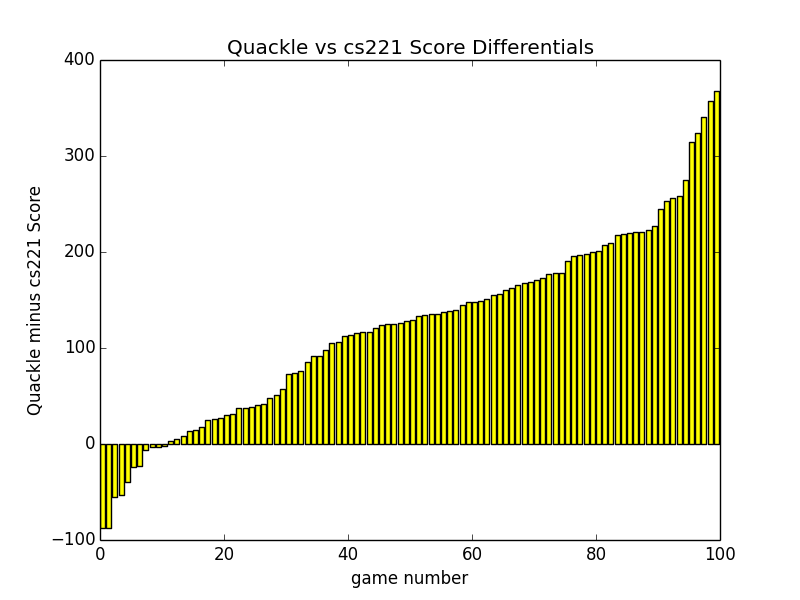
\includegraphics[scale=0.4]{../images/quacklegame_vanilla_100}
  \caption{Quackle vs CS221 Vanilla}
  \endminipage
  \minipage{0.5\textwidth}
      \centering
  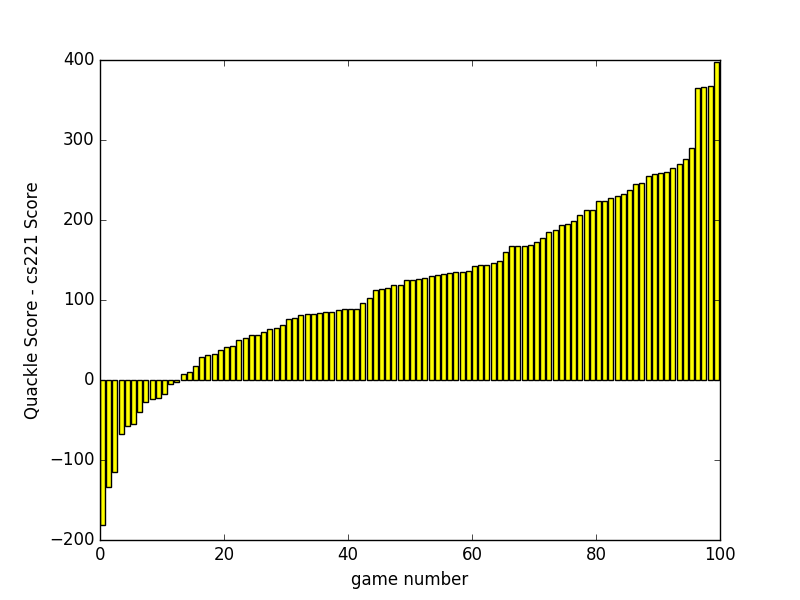
\includegraphics[scale=0.4]{../images/quacklegame_rackH_100}\\
   \caption{Quackle vs CS221 with Rack Heuristics}
  \endminipage{}
\end{figure}

\begin{table}[h]
  \centering
  \begin{tabular}{c|l|l|l|l|l|l}
    \textbf{} & \textbf{win rate} & \textbf{mean} & \textbf{opp mean} & \textbf{mean delta} &  \textbf{2x loss rate} & \textbf{max win ratio} \\\hline
  \textbf{vanilla}   & 11\% & 284.68 & 407.43 & 122.75 & 13\% & 1.358\\
  \textbf{RH}        & 13\% & 288.07 & 410.0  & 121.93 & 11\% & 2.131 \\
  \textbf{MC}        & -    & -      & -      & -      & -    & - \\
  \textbf{MC w/ RH}  & -    & -      & -      & -      & -    & - \\
\end{tabular}
  \caption{Statistics of our AI variants against Quackle's Speedy
    Player. \emph{Mean delta} is the average difference between
    opponent and our score, \emph{2x loss rate} is the rate at which
    the opponent scores 2x or higher, and \emph{max win ratio} is the
    max ratio of our score to opponent's.}
\end{table}

We win 13\% of the time against a world class AI, not bad! Rack
heuristics help slightly, doesn't seem statistically significant. MC
TBD 

\begin{table}[h]
  \centering
  \begin{tabular}{c|l|l|l|l|l|l}
    \textbf{} & \textbf{win rate} & \textbf{mean} & \textbf{opp mean} & \textbf{mean delta} &  \textbf{2x loss rate} & \textbf{max win ratio} \\\hline
  \textbf{control}   & 47\% & 354.24 & 359.25 & -5.01  & 0\%  & 1.811\\
  \textbf{RH}        & 48\% & 351.59 & 353.81 & -2.22  & 0\%  & 1.509\\
  \textbf{MC}        & -    & -      & -      & -      & -    & - \\
  \textbf{MC w/ RH}  & -    & -      & -      & -      & -    & - \\
\end{tabular}
  \caption{Statistics of our AI playing against itself for 300
    games. Control is the vanilla variant playing against itself, all
    other rows are variations playing against vanilla. For description
    of columns, see caption for Table 1.}
\end{table}

As expected, the win rate for the control is about 50/50. The rack
heuristics perform similarly, which is disappointing but not
surprising. The weight vectors, which can be found at the top of
util.py, weighs the raw score multiple orders of magnitude higher than
any other feature. This means that the moves selected in the vanilla
case and the rack heuristic case will not often differ.

The Monte Carlo....[FINISH ME LATER]

Anecdotally, the AI does very well against average humans (the authors and their friends), but the data for this case is difficult and time consuming to collect.

\section*{Conclusion}
Considering we are 2 people who are AI n00bs that had 6 weeks to build an AI in their spare time, and that we manage to beat quackle 13\% of the time...that seems pretty alright!

\clearpage
\begin{center}
 \section*{Code Appendix}
\end{center}
describe code tree

\clearpage
\begin{center}
\section*{Image Appendix}

From Appel-Jacobsen '86\\
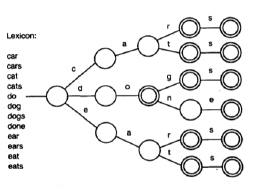
\includegraphics[scale=0.6]{../images/trie}\\
Figure 3: An Example of a Trie \\
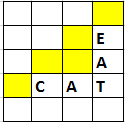
\includegraphics{../images/anchorexample}\\
Figure 4: An Example of Anchor Squares

\vspace{ 8cm }
{\Large References} 
\end{center}
A.W. Appel, G.J. Jacobson, The world’s fastest Scrabble program, Comm. ACM 31 (5) (1988) 572–578, 585. \\
Mark Richards and Eyal Amir. Opponent Modeling in Scrabble. IJCAI-07., 1482–1487, 2007. \\
Stuart Russell and Peter Norvig. Artificial Intelligence: A Modern Approach. Prentice-Hall,
Englewood Cliffs, NJ, 2nd edition edition, 2003 \\
Brian Sheppard. World-championship caliber Scrabble. Artif. Intell., 134:241–245, 2002. \\
J. Katz-Brown, J. O'Laughlin, J. Fultz, M. Liberty, A. Buddhdev, Quackle, http://people.csail.mit.edu/jasonkb/quackle/
\end{document}
